\documentclass{standalone}

\usepackage{tikz}
\usepackage{amsmath}
\usepackage{amssymb}
\usetikzlibrary{positioning,arrows.meta,calc}

\begin{document}

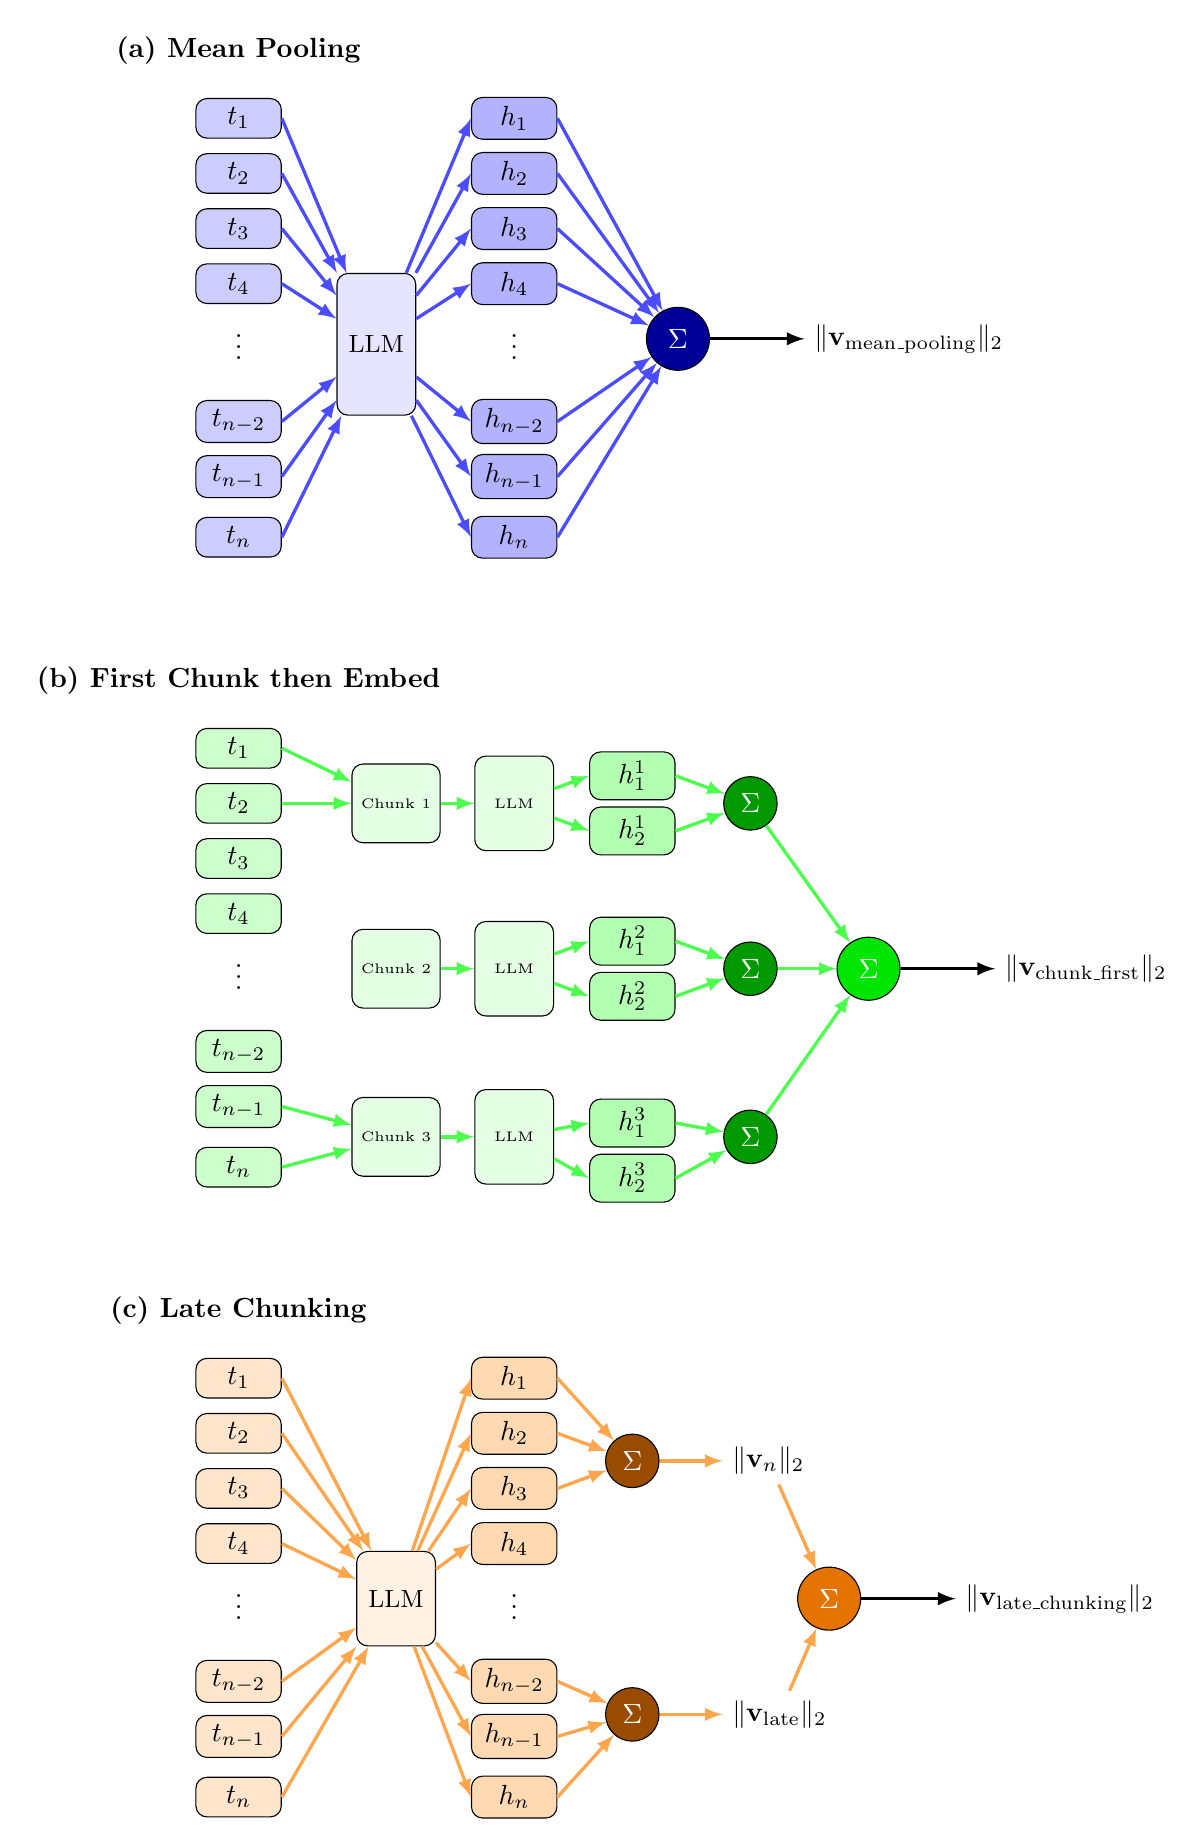
\begin{tikzpicture}[>=latex, node distance=0.8cm]

% Set tighter bounding box to reduce left margin

% -----------------------------------------------------
%  (a) MEAN POOLING
% -----------------------------------------------------
% Tokens at the top
\def\toptokens{4}
\foreach \i in {1,...,\toptokens}{
  \node[draw, fill=blue!20, rounded corners, minimum width=0.9cm, minimum height=0.5cm,
        align=center, text width=0.85cm] (ta\i) at (0,{-(\i-1)*0.7cm}) {$t_{\i}$};
}

% Ellipsis to indicate more tokens
\node[align=center] (ellipsis) at (0,{-(\toptokens)*0.7cm}) {$\vdots$};

% Tokens at the bottom (symmetrical: t_{n-2}, t_{n-1}, t_n) - more vertical spacing
\node[draw, fill=blue!20, rounded corners, minimum width=0.9cm, minimum height=0.5cm,
      align=center, text width=0.85cm] (tanm2) at (0,{-(\toptokens+1.5)*0.7cm}) {$t_{n-2}$};
\node[draw, fill=blue!20, rounded corners, minimum width=0.9cm, minimum height=0.5cm,
      align=center, text width=0.85cm] (tanm1) at (0,{-(\toptokens+2.5)*0.7cm}) {$t_{n-1}$};
\node[draw, fill=blue!20, rounded corners, minimum width=0.9cm, minimum height=0.5cm,
      align=center, text width=0.85cm] (tan) at (0,{-(\toptokens+3.6)*0.7cm}) {$t_n$};

% LLM box in the middle (taller and centered vertically between tokens and hidden states)
% Center it between top token and bottom token (moved higher)
\pgfmathsetmacro{\llmcenterY}{-(\toptokens+0.1)*0.7}
\node[draw, fill=blue!10, rounded corners, minimum width=1.0cm, minimum height=1.8cm,
      align=center] (llmA) at (1.75cm,\llmcenterY cm) {\small LLM};

% Hidden states parallel to tokens (further from LLM)
\foreach \i in {1,...,\toptokens}{
  \node[draw, fill=blue!30, rounded corners, minimum width=0.9cm, minimum height=0.5cm,
        align=center, text width=0.85cm] (ha\i) at (3.5cm,{-(\i-1)*0.7cm}) {$h_{\i}$};
}

% Ellipsis for hidden states
\node[align=center] (ellipsisH) at (3.5cm,{-(\toptokens)*0.7cm}) {$\vdots$};

% Hidden states at the bottom (matching token spacing)
\node[draw, fill=blue!30, rounded corners, minimum width=0.9cm, minimum height=0.5cm,
      align=center, text width=0.85cm] (hanm2) at (3.5cm,{-(\toptokens+1.5)*0.7cm}) {$h_{n-2}$};
\node[draw, fill=blue!30, rounded corners, minimum width=0.9cm, minimum height=0.5cm,
      align=center, text width=0.85cm] (hanm1) at (3.5cm,{-(\toptokens+2.5)*0.7cm}) {$h_{n-1}$};
\node[draw, fill=blue!30, rounded corners, minimum width=0.9cm, minimum height=0.5cm,
      align=center, text width=0.85cm] (han) at (3.5cm,{-(\toptokens+3.6)*0.7cm}) {$h_n$};

% Mean pooling symbol after hidden states
\node[circle, draw, fill=blue!60!black, text=white, minimum size=0.8cm,
      right=1.5cm of ellipsisH] (meanA) {$\Sigma$};

% Arrows from tokens to LLM (exit from right side of tokens)
\foreach \i in {1,...,\toptokens}{
  \draw[->, blue!70, very thick] (ta\i.east) -- (llmA);
}
\draw[->, blue!70, very thick] (tanm2.east) -- (llmA);
\draw[->, blue!70, very thick] (tanm1.east) -- (llmA);
\draw[->, blue!70, very thick] (tan.east) -- (llmA);

% Arrows from LLM to hidden states (enter from left side of hidden states)
\foreach \i in {1,...,\toptokens}{
  \draw[->, blue!70, very thick] (llmA) -- (ha\i.west);
}
\draw[->, blue!70, very thick] (llmA) -- (hanm2.west);
\draw[->, blue!70, very thick] (llmA) -- (hanm1.west);
\draw[->, blue!70, very thick] (llmA) -- (han.west);

% Arrows from hidden states to mean (exit from right side of hidden states)
\foreach \i in {1,...,\toptokens}{
  \draw[->, blue!70, very thick] (ha\i.east) -- (meanA);
}
\draw[->, blue!70, very thick] (hanm2.east) -- (meanA);
\draw[->, blue!70, very thick] (hanm1.east) -- (meanA);
\draw[->, blue!70, very thick] (han.east) -- (meanA);

% Output on the right (with L2 norm)
\node[right=1.2cm of meanA] (outA) {$\|\mathbf{v}_{\text{mean\_pooling}}\|_2$};
\draw[->, very thick] (meanA) -- (outA);

% Title
\node[above=0.3cm of ta1, anchor=south] {\textbf{(a) Mean Pooling}};

% -----------------------------------------------------
%  (b) FIRST CHUNK THEN EMBED
% -----------------------------------------------------
% Y offset for second subplot (below first)
\def\yoffsetB{-8cm}

% Tokens at the top
\foreach \i in {1,...,\toptokens}{
  \node[draw, fill=green!20, rounded corners, minimum width=0.9cm, minimum height=0.5cm,
        align=center, text width=0.85cm] (tb\i) at (0,{\yoffsetB-(\i-1)*0.7cm}) {$t_{\i}$};
}

% Ellipsis to indicate more tokens
\node[align=center] (ellipsisB) at (0,{\yoffsetB-(\toptokens)*0.7cm}) {$\vdots$};

% Tokens at the bottom (symmetrical: t_{n-2}, t_{n-1}, t_n) - matching spacing
\node[draw, fill=green!20, rounded corners, minimum width=0.9cm, minimum height=0.5cm,
      align=center, text width=0.85cm] (tbnm2) at (0,{\yoffsetB-(\toptokens+1.5)*0.7cm}) {$t_{n-2}$};
\node[draw, fill=green!20, rounded corners, minimum width=0.9cm, minimum height=0.5cm,
      align=center, text width=0.85cm] (tbnm1) at (0,{\yoffsetB-(\toptokens+2.5)*0.7cm}) {$t_{n-1}$};
\node[draw, fill=green!20, rounded corners, minimum width=0.9cm, minimum height=0.5cm,
      align=center, text width=0.85cm] (tbn) at (0,{\yoffsetB-(\toptokens+3.6)*0.7cm}) {$t_n$};

% Chunking: Show 3 chunks (simplified representation)
% Chunk 1: tokens t1-t2
\node[draw, fill=green!10, rounded corners, minimum width=1.0cm, minimum height=1.0cm,
      align=center] (chunk1) at ($(2.0cm,{\yoffsetB-1*0.7cm})$) {\tiny Chunk 1};
% Chunk 2: middle tokens
\node[draw, fill=green!10, rounded corners, minimum width=1.0cm, minimum height=1.0cm,
      align=center] (chunk2) at ($(2.0cm,{\yoffsetB-(\toptokens)*0.7cm})$) {\tiny Chunk 2};
% Chunk 3: tokens t_{n-1}-t_n
\node[draw, fill=green!10, rounded corners, minimum width=1.0cm, minimum height=1.0cm,
      align=center] (chunk3) at ($(2.0cm,{\yoffsetB-(\toptokens+3.05)*0.7cm})$) {\tiny Chunk 3};

% LLMs for each chunk
\node[draw, fill=green!10, rounded corners, minimum width=1.0cm, minimum height=1.2cm,
      align=center] (llmB1) at ($(3.5cm,{\yoffsetB-1*0.7cm})$) {\tiny LLM};
\node[draw, fill=green!10, rounded corners, minimum width=1.0cm, minimum height=1.2cm,
      align=center] (llmB2) at ($(3.5cm,{\yoffsetB-(\toptokens)*0.7cm})$) {\tiny LLM};
\node[draw, fill=green!10, rounded corners, minimum width=1.0cm, minimum height=1.2cm,
      align=center] (llmB3) at ($(3.5cm,{\yoffsetB-(\toptokens+3.05)*0.7cm})$) {\tiny LLM};

% Hidden states per chunk (simplified - show a few)
\node[draw, fill=green!30, rounded corners, minimum width=0.9cm, minimum height=0.5cm,
      align=center, text width=0.85cm] (hb1) at ($(5.0cm,{\yoffsetB-0.5*0.7cm})$) {$h_1^1$};
\node[draw, fill=green!30, rounded corners, minimum width=0.9cm, minimum height=0.5cm,
      align=center, text width=0.85cm] (hb2) at ($(5.0cm,{\yoffsetB-1.5*0.7cm})$) {$h_2^1$};

\node[draw, fill=green!30, rounded corners, minimum width=0.9cm, minimum height=0.5cm,
      align=center, text width=0.85cm] (hb3) at ($(5.0cm,{\yoffsetB-(\toptokens-0.5)*0.7cm})$) {$h_1^2$};
\node[draw, fill=green!30, rounded corners, minimum width=0.9cm, minimum height=0.5cm,
      align=center, text width=0.85cm] (hb4) at ($(5.0cm,{\yoffsetB-(\toptokens+0.5)*0.7cm})$) {$h_2^2$};

\node[draw, fill=green!30, rounded corners, minimum width=0.9cm, minimum height=0.5cm,
      align=center, text width=0.85cm] (hb5) at ($(5.0cm,{\yoffsetB-(\toptokens+2.8)*0.7cm})$) {$h_1^3$};
\node[draw, fill=green!30, rounded corners, minimum width=0.9cm, minimum height=0.5cm,
      align=center, text width=0.85cm] (hb6) at ($(5.0cm,{\yoffsetB-(\toptokens+3.8)*0.7cm})$) {$h_2^3$};

% Pooling per chunk
\node[circle, draw, fill=green!60!black, text=white, minimum size=0.6cm] (poolB1) at ($(6.5cm,{\yoffsetB-1*0.7cm})$) {$\Sigma$};
\node[circle, draw, fill=green!60!black, text=white, minimum size=0.6cm] (poolB2) at ($(6.5cm,{\yoffsetB-(\toptokens)*0.7cm})$) {$\Sigma$};
\node[circle, draw, fill=green!60!black, text=white, minimum size=0.6cm] (poolB3) at ($(6.5cm,{\yoffsetB-(\toptokens+3.05)*0.7cm})$) {$\Sigma$};

% Final aggregation (moved to the right of pooling nodes)
\node[circle, draw, fill=green!90!black, text=white, minimum size=0.8cm] (aggB) at ($(8.0cm,{\yoffsetB-(\toptokens)*0.7cm})$) {$\Sigma$};

% Output (with L2 norm)
\node[right=1.2cm of aggB] (outB) {$\|\mathbf{v}_{\text{chunk\_first}}\|_2$};

% Arrows: tokens to chunks
\draw[->, green!70, very thick] (tb1.east) -- (chunk1);
\draw[->, green!70, very thick] (tb2.east) -- (chunk1);
% Removed arrow from ellipsisB to chunk2
\draw[->, green!70, very thick] (tbnm1.east) -- (chunk3);
\draw[->, green!70, very thick] (tbn.east) -- (chunk3);

% Arrows: chunks to LLMs
\draw[->, green!70, very thick] (chunk1) -- (llmB1);
\draw[->, green!70, very thick] (chunk2) -- (llmB2);
\draw[->, green!70, very thick] (chunk3) -- (llmB3);

% Arrows: LLMs to hidden states
\draw[->, green!70, very thick] (llmB1) -- (hb1.west);
\draw[->, green!70, very thick] (llmB1) -- (hb2.west);
\draw[->, green!70, very thick] (llmB2) -- (hb3.west);
\draw[->, green!70, very thick] (llmB2) -- (hb4.west);
\draw[->, green!70, very thick] (llmB3) -- (hb5.west);
\draw[->, green!70, very thick] (llmB3) -- (hb6.west);

% Arrows: hidden states to pooling
\draw[->, green!70, very thick] (hb1.east) -- (poolB1);
\draw[->, green!70, very thick] (hb2.east) -- (poolB1);
\draw[->, green!70, very thick] (hb3.east) -- (poolB2);
\draw[->, green!70, very thick] (hb4.east) -- (poolB2);
\draw[->, green!70, very thick] (hb5.east) -- (poolB3);
\draw[->, green!70, very thick] (hb6.east) -- (poolB3);

% Arrows: pooling to final aggregation
\draw[->, green!70, very thick] (poolB1) -- (aggB);
\draw[->, green!70, very thick] (poolB2) -- (aggB);
\draw[->, green!70, very thick] (poolB3) -- (aggB);

% Arrow: aggregation to output
\draw[->, very thick] (aggB) -- (outB);

% Title
\node[above=0.3cm of tb1, anchor=south] {\textbf{(b) First Chunk then Embed}};

% -----------------------------------------------------
%  (c) LATE CHUNKING
% -----------------------------------------------------
% Y offset for third subplot (below second)
\def\yoffsetC{-16cm}

% Tokens at the top
\foreach \i in {1,...,\toptokens}{
  \node[draw, fill=orange!20, rounded corners, minimum width=0.9cm, minimum height=0.5cm,
        align=center, text width=0.85cm] (tc\i) at (0,{\yoffsetC-(\i-1)*0.7cm}) {$t_{\i}$};
}

% Ellipsis to indicate more tokens
\node[align=center] (ellipsisC) at (0,{\yoffsetC-(\toptokens)*0.7cm}) {$\vdots$};

% Tokens at the bottom (symmetrical: t_{n-2}, t_{n-1}, t_n) - matching spacing
\node[draw, fill=orange!20, rounded corners, minimum width=0.9cm, minimum height=0.5cm,
      align=center, text width=0.85cm] (tcnm2) at (0,{\yoffsetC-(\toptokens+1.5)*0.7cm}) {$t_{n-2}$};
\node[draw, fill=orange!20, rounded corners, minimum width=0.9cm, minimum height=0.5cm,
      align=center, text width=0.85cm] (tcnm1) at (0,{\yoffsetC-(\toptokens+2.5)*0.7cm}) {$t_{n-1}$};
\node[draw, fill=orange!20, rounded corners, minimum width=0.9cm, minimum height=0.5cm,
      align=center, text width=0.85cm] (tcn) at (0,{\yoffsetC-(\toptokens+3.6)*0.7cm}) {$t_n$};

% LLM box (single LLM like mean pooling)
\node[draw, fill=orange!10, rounded corners, minimum width=1.0cm, minimum height=1.2cm,
      align=center] (llmC) at ($(2.0cm,{\yoffsetC-(\toptokens)*0.7cm})$) {\small LLM};

% Hidden states parallel to tokens (like mean pooling)
\foreach \i in {1,...,\toptokens}{
  \node[draw, fill=orange!30, rounded corners, minimum width=0.9cm, minimum height=0.5cm,
        align=center, text width=0.85cm] (hc\i) at ($(3.5cm,{\yoffsetC-(\i-1)*0.7cm})$) {$h_{\i}$};
}

% Ellipsis for hidden states
\node[align=center] (ellipsisHC) at ($(3.5cm,{\yoffsetC-(\toptokens)*0.7cm})$) {$\vdots$};

% Hidden states at the bottom (matching token spacing)
\node[draw, fill=orange!30, rounded corners, minimum width=0.9cm, minimum height=0.5cm,
      align=center, text width=0.85cm] (hcnm2) at ($(3.5cm,{\yoffsetC-(\toptokens+1.5)*0.7cm})$) {$h_{n-2}$};
\node[draw, fill=orange!30, rounded corners, minimum width=0.9cm, minimum height=0.5cm,
      align=center, text width=0.85cm] (hcnm1) at ($(3.5cm,{\yoffsetC-(\toptokens+2.5)*0.7cm})$) {$h_{n-1}$};
\node[draw, fill=orange!30, rounded corners, minimum width=0.9cm, minimum height=0.5cm,
      align=center, text width=0.85cm] (hcn) at ($(3.5cm,{\yoffsetC-(\toptokens+3.6)*0.7cm})$) {$h_n$};

% Windowed pooling: Show 2 windows (overlapping)
% Window 1: top hidden states
\node[circle, draw, fill=orange!60!black, text=white, minimum size=0.6cm] (poolC1) at ($(5.0cm,{\yoffsetC-1.5*0.7cm})$) {$\Sigma$};
% Window 2: bottom hidden states  
\node[circle, draw, fill=orange!60!black, text=white, minimum size=0.6cm] (poolC2) at ($(5.0cm,{\yoffsetC-(\toptokens+2.1)*0.7cm})$) {$\Sigma$};

% Window vectors with L2 norm notation
\node[right=0.8cm of poolC1] (vecC1) {$\|\mathbf{v}_n\|_2$};
\node[right=0.8cm of poolC2] (vecC2) {$\|\mathbf{v}_{\text{late}}\|_2$};

% Final aggregation (moved to the right of window vectors)
\node[circle, draw, fill=orange!90!black, text=white, minimum size=0.8cm] (aggC) at ($(7.5cm,{\yoffsetC-(\toptokens)*0.7cm})$) {$\Sigma$};

% Output (with L2 norm)
\node[right=1.2cm of aggC] (outC) {$\|\mathbf{v}_{\text{late\_chunking}}\|_2$};

% Arrows from tokens to LLM (exit from right side)
\foreach \i in {1,...,\toptokens}{
  \draw[->, orange!70, very thick] (tc\i.east) -- (llmC);
}
\draw[->, orange!70, very thick] (tcnm2.east) -- (llmC);
\draw[->, orange!70, very thick] (tcnm1.east) -- (llmC);
\draw[->, orange!70, very thick] (tcn.east) -- (llmC);

% Arrows from LLM to hidden states (enter from left side)
\foreach \i in {1,...,\toptokens}{
  \draw[->, orange!70, very thick] (llmC) -- (hc\i.west);
}
\draw[->, orange!70, very thick] (llmC) -- (hcnm2.west);
\draw[->, orange!70, very thick] (llmC) -- (hcnm1.west);
\draw[->, orange!70, very thick] (llmC) -- (hcn.west);

% Arrows from hidden states to windowed pooling (exit from right side)
% Window 1: connects to top hidden states
\draw[->, orange!70, very thick] (hc1.east) -- (poolC1);
\draw[->, orange!70, very thick] (hc2.east) -- (poolC1);
\draw[->, orange!70, very thick] (hc3.east) -- (poolC1);
% Window 2: connects to bottom hidden states
\draw[->, orange!70, very thick] (hcnm2.east) -- (poolC2);
\draw[->, orange!70, very thick] (hcnm1.east) -- (poolC2);
\draw[->, orange!70, very thick] (hcn.east) -- (poolC2);

% Arrows from pooling to window vectors
\draw[->, orange!70, very thick] (poolC1) -- (vecC1);
\draw[->, orange!70, very thick] (poolC2) -- (vecC2);

% Arrows from window vectors to final aggregation
\draw[->, orange!70, very thick] (vecC1) -- (aggC);
\draw[->, orange!70, very thick] (vecC2) -- (aggC);

% Arrow: aggregation to output
\draw[->, very thick] (aggC) -- (outC);

% Title
\node[above=0.3cm of tc1, anchor=south] {\textbf{(c) Late Chunking}};

\end{tikzpicture}


\end{document}